%%%%%%%%%%%%%%%%%%%%%%%%%%%%%%%% FIXED 
\documentclass[11pt]{article}
\usepackage{graphicx}
\pagestyle{empty}
\setlength{\parskip}{0.25\baselineskip}
\renewcommand{\title}[1]{{\noindent\large\bfseries#1\medskip\\}}
\renewcommand{\author}[2]{{\noindent #1 \medskip\\ \small #2 \medskip\\}}
\renewcommand\refname{}
\usepackage[letterpaper,margin=20mm]{geometry}
\usepackage{hyperref}
%%%%%%%%%%%%%%%%%%%%%%%%%%%%%%%%

\begin{document}

\title{Crowdsourcing ground-truth datasets for building change detection}
\author{
% Authors Names
Juste Raimbault,\textsuperscript{1,2,3,4}
Julien Perret,\textsuperscript{1,5}
}
{
% Authors Affiliations
1. LaSTIG, Univ. Gustave Eiffel, IGN-ENSG\\
2. CASA, UCL\\
3. UPS CNRS 3611 ISC-PIF\\
4. UMR CNRS 8504 G{\'e}ographie-cit{\'e}s\\
5. LaDéHiS, EHESS
}


% [23/03] TODO avant le 05/04 : edits? -> au moins clarifier le "optimised" vs "trained"
% [23/03] Paper annotator ? Ijgis (t and f) ? [Thgt hier // sch bib ce journal]


% mini abstract 2000 caracs
% A quantification of urban densification is necessary at the building level to explore sustainable policies linked to densification processes, because of the multiple stakeholders involved at several scales. To that end, geospatial vector data matching algorithms are a powerful tool to detect building change, but lack ground-truth datasets for their optimisation. We introduce a web application to crowdsource the annotation of vector data matching links, implemented on building data at two different dates. Preliminary annotated datasets are used to test the performance of two algorithms previously optimised on synthetic data. Our contribution thus provide a basis for a robust quantification of urban densification at the building level, and a generic web application to annotate vector datasets in a comparative way.


% ABSTRACT

An accurate quantification of past urban dynamics is key for designing future sustainable cities \cite{batty2018inventing}. More particularly, dynamics of urban densification are a complex yet crucial issue, since they link to several conflicting sustainability goals \cite{evers2024urbanization} (e.g. increased access to public transport and amenities, and limited urban sprawl, but with negative externalities such as less urban green space or an increased urban heat island effect), and imply several stakeholders at multiple scales what makes these difficult to control through policies \cite{jehling2020densification}. Since landowners are often implied in plot splitting or soft densification, an understanding of change dynamics is required at the building level. Raster data such as aerial imagery, on which machine learning methods provide a good performance for land-use change for example \cite{khelifi2020deep}, is not sufficient for that purpose, and change detection must be performed on vector data of building geometries. To that purpose, geospatial vector data matching algorithms are an efficient tool \cite{xavier2016survey}, with the advantage of being robust to spatial noise in geometries and changes in data specifications. They however require some extensive parametrisation and provide varying performances \cite{guardiola2024optimising}. An important issue for optimising this type of algorithms is the lack of ground-truth datasets with a large enough size and diversity. We propose in this contribution to tackle this issue, for the specific case of building change detection.

We therefore introduce a web application designed to annotate potential matching links between two vector datasets. Its main functionalities are that (i) it is fully based on git and javascript, requiring no database nor advanced web server deployment, and can be automatically deployed through github pages for example; (ii) it manages multi-user collaboration, with authentication linked to rights granted for the project git repository (implemented only for github for now); (iii) provides a dashboard with the user progress and the overall progress on all datasets displayed on maps; (iv) it allows collaborators annotating two vector datasets at two different dates, with aerial photographs being provided in the background for ground-truthing. The annotation is sequential on potential matching links (intersecting features between the two datasets), and the user must ground-truth first the type of link the algorithm should detect (no link, single, multiple), then the type of real world evolution (parametrised for building changes in our case), and can also highlight and comment data quality issues. The application is open source and available at \url{https://github.com/subdense/annotate}.

We show an example of the application in Figure 1. We currently deployed the application on samples within the functional urban areas of Strasbourg, France and Dortmund, Germany, as data quality issues are very different across countries (for example, French BDTopo had a specification change in 2015 leading to many geometry changes with polygon splits that do not correspond to real-world changes). We compare buildings between 2011 and 2021, for all buildings within 500m radius circles around 100 sampled points for each area. The annotation campaign is currently ongoing with several researchers experts on GIS data and urban densification. First results to optimise algorithms (in the sense of F-score for real-world change prediction) with partial ground-truth datasets were obtained for the same algorithms studied by \cite{guardiola2024optimising} (the Multi-criteria matching algorithm and the Geometric Matching of Areas algorithm), and confirm previous results obtained with synthetic data, in particular that (i) each algorithm can be optimised to better perform in different urban form typologies (center, housing projects, suburbs); (ii) they can be combined into a multi-modelling approach for a better overall performance.

Our contribution thus provide a basis for a robust quantification of urban densification at the building level, and a generic web application to annotate vector datasets in a comparative way.

\newpage


\begin{figure}%[b]
  \centering
  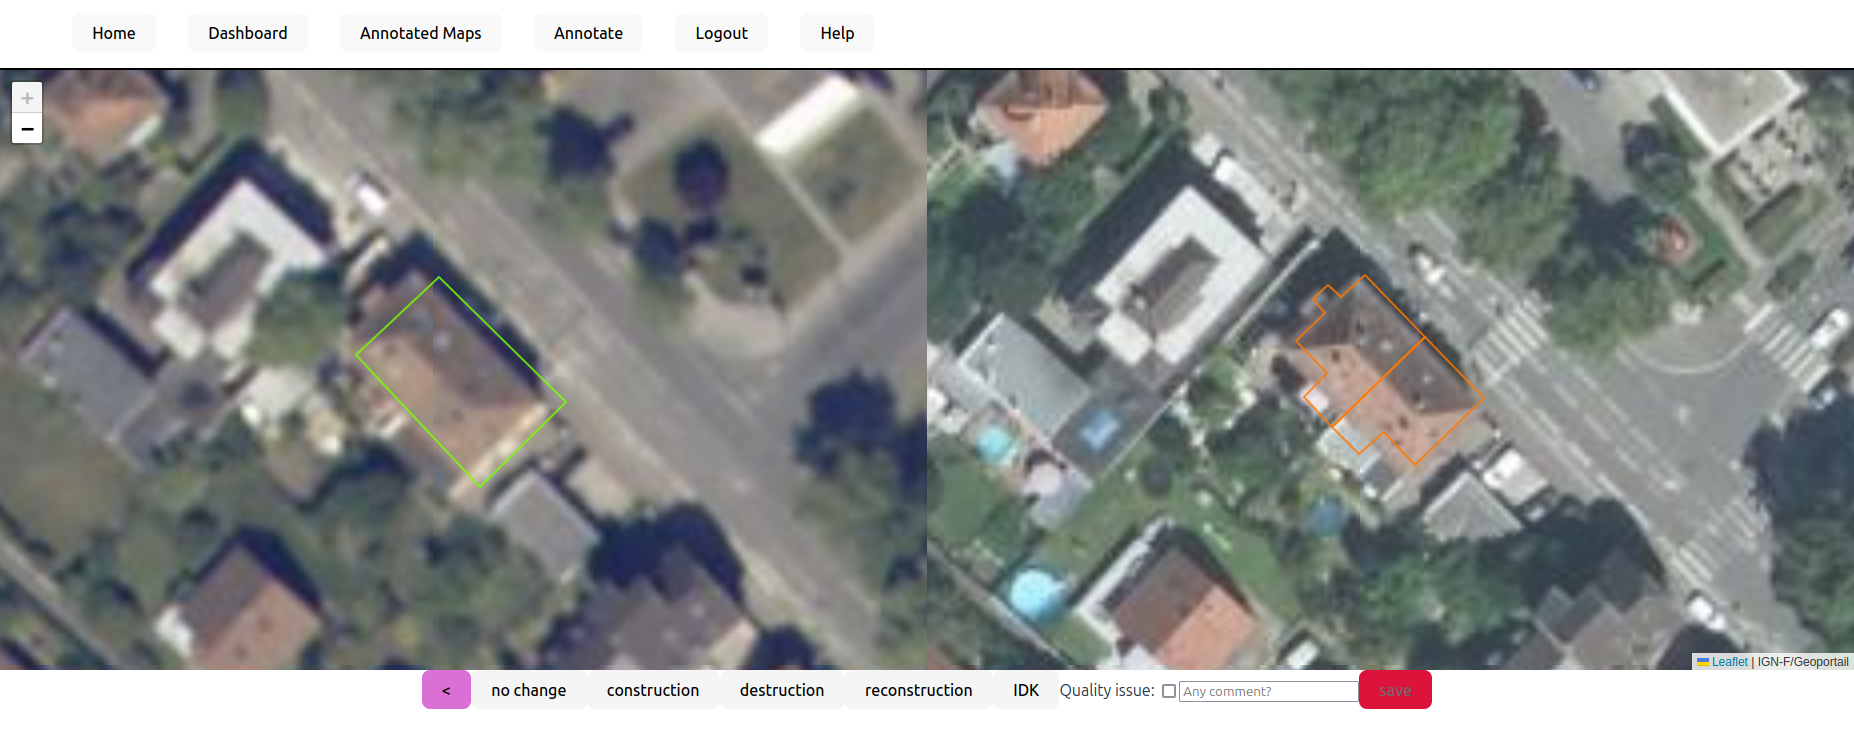
\includegraphics[width=\textwidth]{figures/example_annotate_2025-03-20_22-27-20.png}
  \caption{Screenshot of the annotation web application. On the top the user can access the different tabs, such as the dashboard with the annotation progress on the tasks ths user was assigned, or global maps showing progress across all users and datasets in space. The main tab to annotate shows two aerial photographs of the same place at the two compared dates, with the vector features at each date surimposed. In this particular case, there seems to be no change in the real world, but the polygon data for buildings significantly changed. The user first provides the type of link, and then (shown in the screenshot) the type of real world building change (no change, construction, destruction, reconstruction, does not know), and can comment on a data quality issue. Note that aerial photographs are in some rare cases not enough to ground-truth change, thus the option to skip the step. Once clicking ``save'', the next unit to annotate will be displayed. The application is currently parametrised for building change, but vector data sources, aerial imagery sources, and change labels can all be customised in a configuration file, and thus can be changed for other types of features, such as land plots or road networks.}
\end{figure}

{\small
%\linespread{1}\selectfont
\bibliographystyle{unsrt}
\bibliography{biblio}
}

\end{document}




%\bigskip
%{\small
%\noindent[1] Here you can add references.\\
%\noindent[2] Differently from this one, not written using a LLM.
%}

%\begin{figure}[b]
%  \centering
%  \includegraphics[width=0.5\textwidth]{figure.pdf}
%  \caption{Figure caption.}
%\end{figure}

